\documentclass[a4paper, 10pt, french]{article}
% Préambule; packages qui peuvent être utiles
   \RequirePackage[T1]{fontenc}        % Ce package pourrit les pdf...
   \RequirePackage{babel,indentfirst}  % Pour les césures correctes,
                                       % et pour indenter au début de chaque paragraphe
   \RequirePackage[utf8]{inputenc}   % Pour pouvoir utiliser directement les accents
                                     % et autres caractères français
   \RequirePackage{lmodern,tgpagella} % Police de caractères
   \textwidth 17cm \textheight 25cm \oddsidemargin -0.24cm % Définition taille de la page
   \evensidemargin -1.24cm \topskip 0cm \headheight -1.5cm % Définition des marges

   \RequirePackage{latexsym}                  % Symboles
   \RequirePackage{amsmath}                   % Symboles mathématiques
   \RequirePackage{tikz}   % Pour faire des schémas
   \RequirePackage{graphicx} % Pour inclure des images
   \RequirePackage{listings} % pour mettre des listings
% Fin Préambule; package qui peuvent être utiles

\title{Rapport de TP 4MMAOD : Génération de patch optimal}
\author{
MAHIEU LUCAS étudiant$_1$ (SLE\_PHELMA$_1$) 
\\ ANOUFA Guillaume étudiant$_2$ (SLE\_PHELMA$_2$) 
}

\begin{document}

\maketitle

%%%%%%%%%%%%%%%%%%%%%%%%%%%%%%%%%%%%%%%%%%%%%%

%%%%%%%%%%%%%%%%%%%%%%%%%%%%%%%%%%%%%%%%%%%%%%
\section{Principe de notre  programme (1 point)}
{Nous avons choisi d'implementer un algorithme itératif car cela nous paraissait plus efficace qu'un algorithme récursif qui aurait du faire un très grand nombre d'appel et potentiellement remplir entièrement la pile, pour des fichiers volumineux.
\\ \indent Ainsi nous parcourons une à une toutes les configurations de fichier possible : de $A_0$,$B_0$ à $A_n$,$B_n$, et mémorisons le cout de la configuration à chaque itération.
\\ \indent Pour pouvoir retrouver, à la fin, par quelle configuration nous sommes arrivé à $A_n$,$B_n$, nous mémorisons aussi les indices de la configuration mère ainsi que le numéro du 1er caractère de la ligne qu'il faudra afficher dans le patch dans le cas ou celui-ci passe par cette configuration.
\\ \indent Pour mémoriser ces informations, nous avons utiliser un tableau de taille (n+1)*(m+1) {\em Mono-dimensionel} qui contient des structures appelées 'cellule'. Ce tableau sera repérée par la variable globale '(cellule*)mem'. Elles sont définies comme ceci:
{\em \\typedef struct  \{
\\ \indent int cout, -> qui correspond au cout pour arriver dans cette configuration.
\\ \indent size\_t l\_cpy, -> qui contiendra le $1_{er}$ octet de la ligne à recopier dans le patch pour les opération '+' et '='.
\\ \indent int pereI, -> qui contient la position i de la cellule ayant donné le coût min pour la cellule en question
\\ \indent int pereJ -> qui contient la position j de la cellule ayant donné le coût min pour la cellule en question\} cellule;}
\\ \indent Pour mieux comprendre nous avons schématiser ce que notre algorithme fait pour l'exemple du sujet. Voir figure~\ref{étiquette} page~\pageref{étiquette} 

\begin{figure}[!h]
\hspace{2cm}
	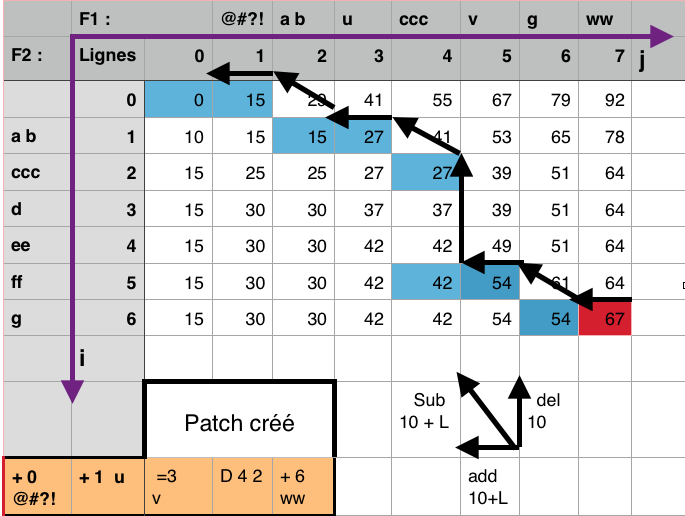
\includegraphics[scale=0.5]{tableau_mem.png}
	\caption{\label{étiquette} Exemple de parcours itératif de notre algorithme pour l'exemple du sujet}
\end{figure}
 \indent Notre algorithme commence dans l'état $A_0$,$B_0$ et calcule colonne par colonne tous les coûts de toutes des configurations. Pour ce faire, à l'étape $A_i$,$B_j$, le coût sera : \\ min \{ ($A_{i-1}$,$B_{j-1}$) + 10+L, ($A_i$,$B_{j-1}$) + 10+L, min\{ ($A_{i-k}$,$B_j$) + 15\} \}
 \\ C'est ce que représente partiellement (sans l'opération 'D') la figure en bas à droite de la figure~\ref{étiquette} page~\pageref{étiquette} 
 \\ \indent Lorsque l'on arrive dans l'état $A_n$,$B_m$, on va remonter le chemin des pères. Donc en $A_i$,$B_j$ on ira en $A_{péreI}$,$B_{péreJ}$ en {\em 'échangeant'} la valeur des pères pour qu'une fois en $A_0$,$B_0$ on puisse redescendre en $A_n$,$B_m$ par le chemin de coût optimal tout en l'affichant.
 \\ \indent De plus, pour améliorer les performances, nous utilisons la commande 'mmap' pour les fichiers F1 et F2, qui permet de lire dans les fichiers en coût constant $\Theta$(1).
 } 

%%%%%%%%%%%%%%%%%%%%%%%%%%%%%%%%%%%%%%%%%%%%%%
\section{Analyse du coût théorique (3 points)}
{\em Donner ici l'analyse du coût théorique de votre programme en fonction des nombres $n_1$ et $n_2$ de lignes 
et $c_1$ et $c_2$ de caractères des deux fichiers en entrée.
 Pour chaque coût, donner la formule qui le caractérise (en justifiant brièvement pourquoi cette formule correspond à votre programme), 
 puis l'ordre du coût en fonction de $n_1, n_2, c_1, c_2$ en notation $\Theta$ de préférence, sinon $O$.}

  \subsection{Nombre  d'opérations en pire cas\,: }
    \paragraph{Justification\,: }
    {Dans le pire cas, il faut remplacer toutes les lignes de F1 par les lignes de F2: 
      \\Le programme itératif contient deux boucles imbriquées $k_1=[0,n_1]$, $k_2=[0,n_2]$ chacune de ces boucles traitent respectivement une lignes des fichiers F1 et F2. Ces deux boucles calcules le nombre de caractères sur leur lignes respectives. Ensuite seule des opérations à coût constants sont réalisées pour calculer le coût minimum et pour créer le 'chemin' idéal. A cela nous ajoutons une somme qui correspond au coût de l'affichage du patch dans le pire cas (écriture de $c_2$ caractère).
      $$T(n_1, n_2, c_1, c_2) = \sum_{k_2=0}^{n_2}  \sum_{k_1=0}^{n_1} (c_1/n_1)*(c_2/n_2) + \sum_{i=0}^{n_2} c_2/n_2 $$ 
      cette somme calculée donne approximativement: $$ T(n_1, n_2, c_1, c_2) = \Theta (c_1*c_2+c_2) = \Theta (c_1*c_2) $$ 
    } 
  \subsection{Place mémoire requise\,: }
    \paragraph{Justification\,: }
    {
    	Comme la partie 1 l'explique, nous stockons en mémoire $(n+1)*(m+1)$ états sachant que 1 état prend un place de $4*sizeof(int)$, nous mémorisons $4*sizeof(int)*(n+1)*(m+1)$ octets.
	\\De plus, en utilisant mmap, nous 'mappons' en mémoire les fichiers d'entrée et de sortie, ainsi nous utilisons $(c1+c2)$ octet de plus. \\Ce qui fait un total de $4*sizeof(int)*(n+1)*(m+1) + (c1+c2)$
    }

  \subsection{Nombre de défauts de cache sur le modèle CO\,: }
    \paragraph{Justification\,: }
    { Nous utilisons deux boucles for imbriquées de telle sorte qu'on parcourt le tableau séquentiellement avec un pas unitaire. On respecte ainsi le principe de localité spatiale et on limite donc le nombre de défauts de cache. D'après la simulation présentée dans le cours, pour un parcours itératif d'un tableau en STRIDE 1 de 1,000,000 de lignes on pouvait observer un nombre de défauts de cache de 378,448. Ici, on s'attendra donc à un résultat similaire (proportionnellement au produit $n_1*n_2$).
    
    La figure~\ref{étiquette} page~\pageref{étiquette} illustre la forme de notre tableau en mémoire. Nos boucles sont créées de la façon suivante : \\ for( j=0; j<$n_2$; j++) \{ \\ \indent for( i=0 ; i< $n_1$; i++)\{ \\ \indent \indent ... Calcul du coût \\ \indent \} \\ \}
	\begin{figure}[!h]
\hspace{1cm}
	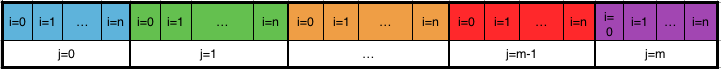
\includegraphics[scale=0.6]{zone_mem.png}
	\caption{\label{étiquette} Zone mémoire allouée}
\end{figure}
    
    }


%%%%%%%%%%%%%%%%%%%%%%%%%%%%%%%%%%%%%%%%%%%%%%
\section{Compte rendu d'expérimentation (2 points)}
  \subsection{Conditions expérimentaless}
  
    \subsubsection{Description synthétique de la machine\,:} 
      {Les tests ont été effectués sur un MacBookPro équipé d'un processeur intel Core 2 Duo (1 processeur à 2 coeurs), de 2,4GHz. La mémoire RAM disponible est de 10Go ainsi que 3Mo de mémoire cache. Le système d'exploitation utilisé est Mac OS X El Capitan 10.11.1. Durant le test aucun autre programme était en cours d'utilisation.
      } 

    \subsubsection{Méthode utilisée pour les mesures de temps\,: } 
      {Les mesures présentées ci dessous ont été effectué grace à a fonction UNIX {\em time}.Les valeurs sont données en secondes et correspondent au temps système, c'est à dire le temps qu'a mis le système à executer le programme. Les tests ont été effectués successivement benchmark par benchmark.
      }

  \subsection{Mesures expérimentales}
  
    \begin{figure}[h]
      \begin{center}
        \begin{tabular}{|l||r||r|r|r||}
          \hline
          \hline
            & coût         & temps     & temps   & temps \\
            & du patch     & min       & max     & moyen \\
          \hline
          \hline
            benchmark1 &2540 &0,023      &0,026     &0,024      \\
          \hline
            benchmark2 &3120      &0,092     &0,100     &0,096     \\
          \hline
            benchmark3 &809      &0,180     &0,181     &0,180     \\
          \hline
            benchmark4 &1708      &0,322     &0,330     &0,326     \\
          \hline
            benchmark5 &7553      &0,503     &0,513     &0,509     \\
          \hline
            benchmark6 &37027      &2,214     &2,240     &2,230     \\
          \hline
          \hline
        \end{tabular}
        \caption{Mesures des temps minimum, maximum et moyen de 5 exécutions pour les 6 benchmarks.(sec)}
        \label{table-temps}
      \end{center}
    \end{figure}

\subsection{Analyse des résultats expérimentaux}
\paragraph{Justification\,: }
	{ 
	On observe un nombre de défauts de cache LL de 407,583 pour 1,314,910 références (pour l'execution de computePatchOpt sur le Benchmark\_01 pour lequel $n_1=1000 et n_2=1047$) (voir figure~\ref{cccc} page~\pageref{cccc}). 
Ceci est donc cohérent avec notre algorithme et nos attentes en comparaison avec le parcours du tableau de 1,000,000 de lignes en STRIDE 1.
    	\begin{figure}[!h]
\hspace{1cm}
	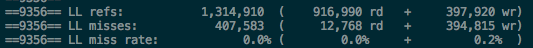
\includegraphics[scale=0.6]{cache_LL.png}
	\caption{\label{cccc} Exemple de parcours itératif de notre algorithme pour l'exemple du sujet}
\end{figure}
     }

%%%%%%%%%%%%%%%%%%%%%%%%%%%%%%%%%%%%%%%%%%%%%%
\section{Question\,: et  si le coût d'un patch était sa taille en octets ? (1 point)}
\paragraph{Justification\,: }
{
Pour ce faire il faudrait changer le coût de chaque opération en le définissant comme le nombre d'octet à afficher dans le patch.
Concrètement cela reviendrait à :
\begin{itemize}
	\item Délétion : coût de 7 car ' d k '  coûte 7 octets si k est un int sur 32 bits
	\item Délétion multiple : coût de 12 car ' D k m ' coûte 12 octets si k et m sont des int sur 32 bits
	\item Addition : coût de 7 + $L_k(B)$ car ' + k ' coûte 7 octets si k est un int sur 32 bits
	\item Substitution : coût de 7 + $L_k(B)$ car ' = k ' coûte 7 octets si k est un int sur 32 bits
\end{itemize}
De cette façon les deletions deviennent plus rentable globalement. On obtient alors le patch de coût minimum en terme de nombre d'octets à écrire dans le patch.

}

\end{document}
%% Fin mise au format

